
\begin{figure}[ht]
    \centering
    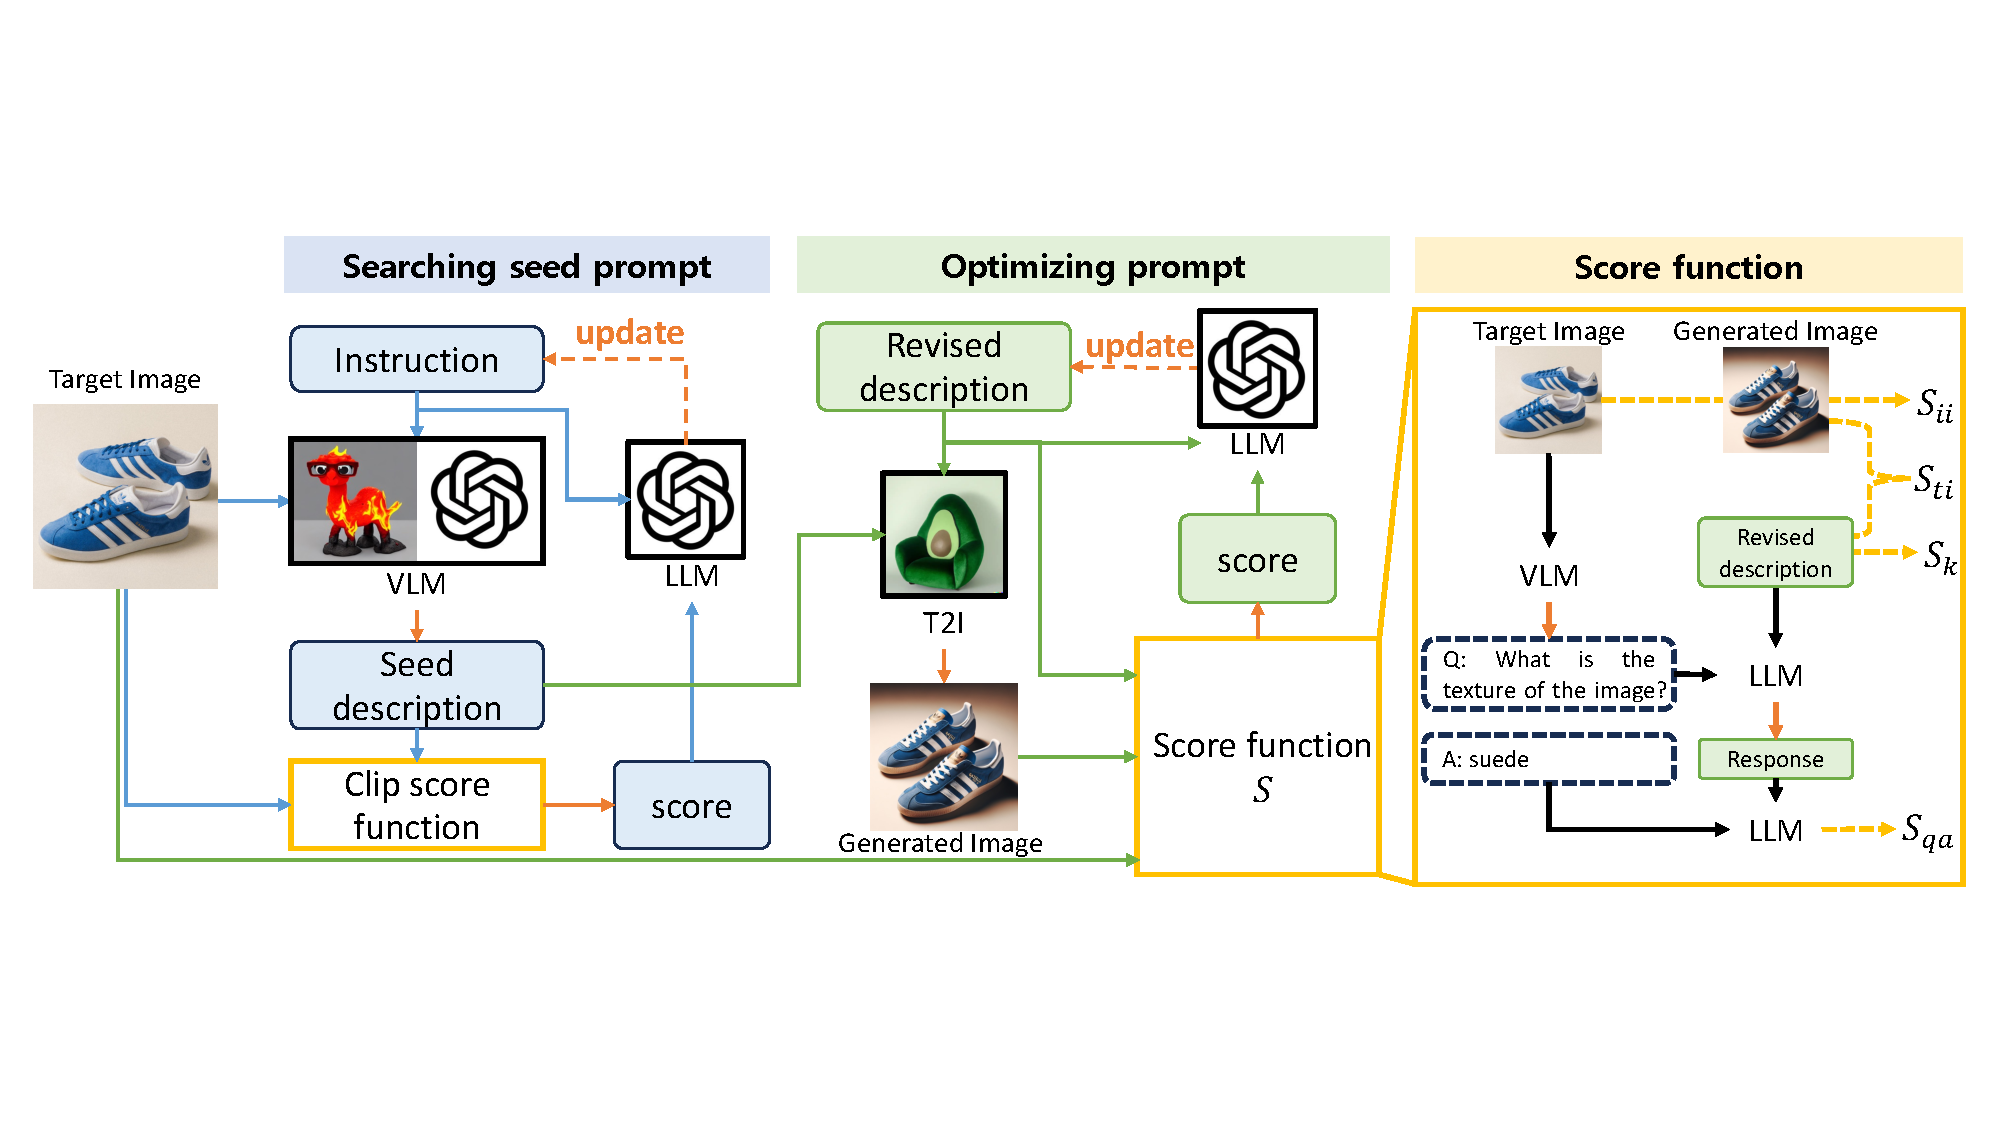
\includegraphics[width=0.99\textwidth]{figure_folder/detail_pipeline.pdf}
    \vspace{-0.1in}
    \caption{\small \textbf{Detailed figure of automated prompt generation pipeline.} The initial step is to optimize the instruction for the vision-large language model (VLM) in order to generate a high-quality seed prompt that is well aligned to the target image in the CLIP space.  Then, in the automated prompt tuning step, the prompt for text-to-image model (T2I) is optimized to generate precise description of the target image. The optimizing score at the automated prompt tuning stage comprises four functions, image-image consistency $S_{ii}$, image-text alignment score $S_{ti}$, keyword penalty $S_k$, and self-generated QA score $S_{qa}$.}
    \label{fig:detail_pipeline}
    \vspace{-0.23in}
\end{figure}